\section{Il gruppo Obelix}
\begin{frame}
	
	\begin{columns}
		\begin{column}{0.2\textwidth}
			
		\end{column}
		
		\begin{column}{0.4\textwidth}
			\begin{itemize}
				\item Emanuele Crespan
				\item Tomas Mali
				\item Silvio Meneguzzo
				\item Nicolò Rigato
				\item Riccardo Saggese
				\item Federica Schifano
			\end{itemize}
		\end{column}
		
		\begin{column}{0.2\textwidth}
			
		\end{column}
	\end{columns}


\end{frame}

\section{Introduzione}
\subsection{Cos'era una bolla?}
\begin{frame}
	\frametitle{Cos'era una bolla?}
	\begin{center}
		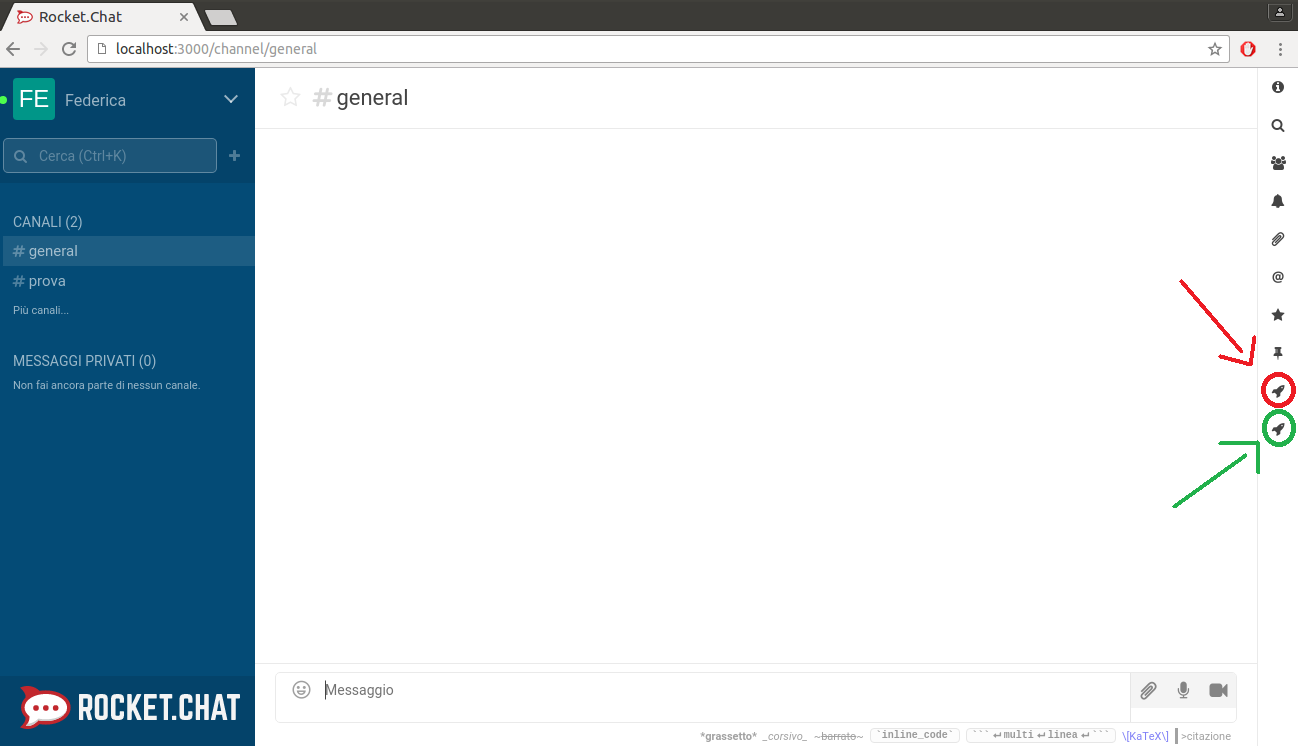
\includegraphics[scale=0.23]{img/f1.png}
	\end{center}
	
\end{frame}

\subsection{Cos'è una bolla?}
\begin{frame}
  \frametitle{Cos'è una bolla?}
  \textbf{Non più un messaggio speciale tra messaggi}
  \begin{center}
  	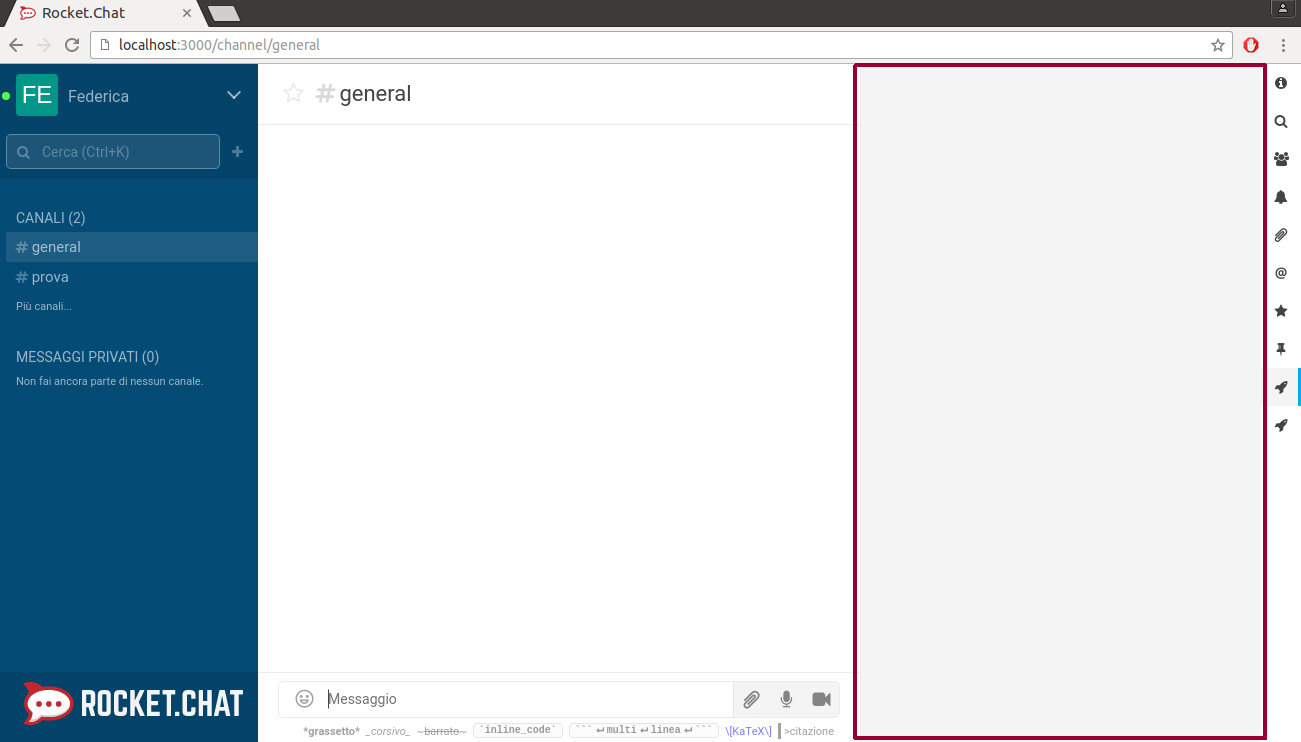
\includegraphics[scale=0.20]{img/f2.png}
  \end{center}

\end{frame}

%\subsection{prova3}
\begin{frame}
  \frametitle{Cos'è una bolla?}
% \framesubtitle{prova}
 \textbf{Un'applicazione eseguita in un'apposita SideArea}
\begin{center}
	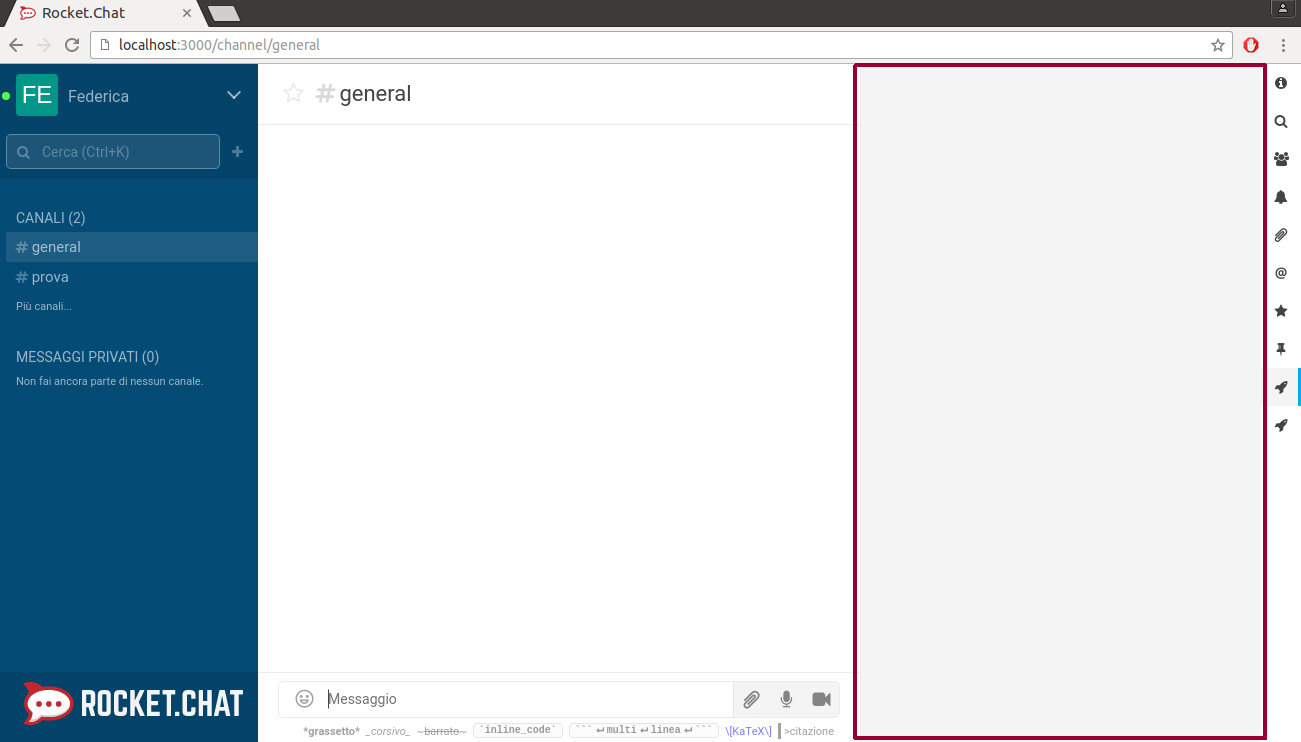
\includegraphics[scale=0.20]{img/f4.png}
\end{center}
 
\end{frame}

\begin{frame}
	\begin{figure}
		\begin{center}
			\caption{Due nuovi pulsanti nella tabbar laterale}
			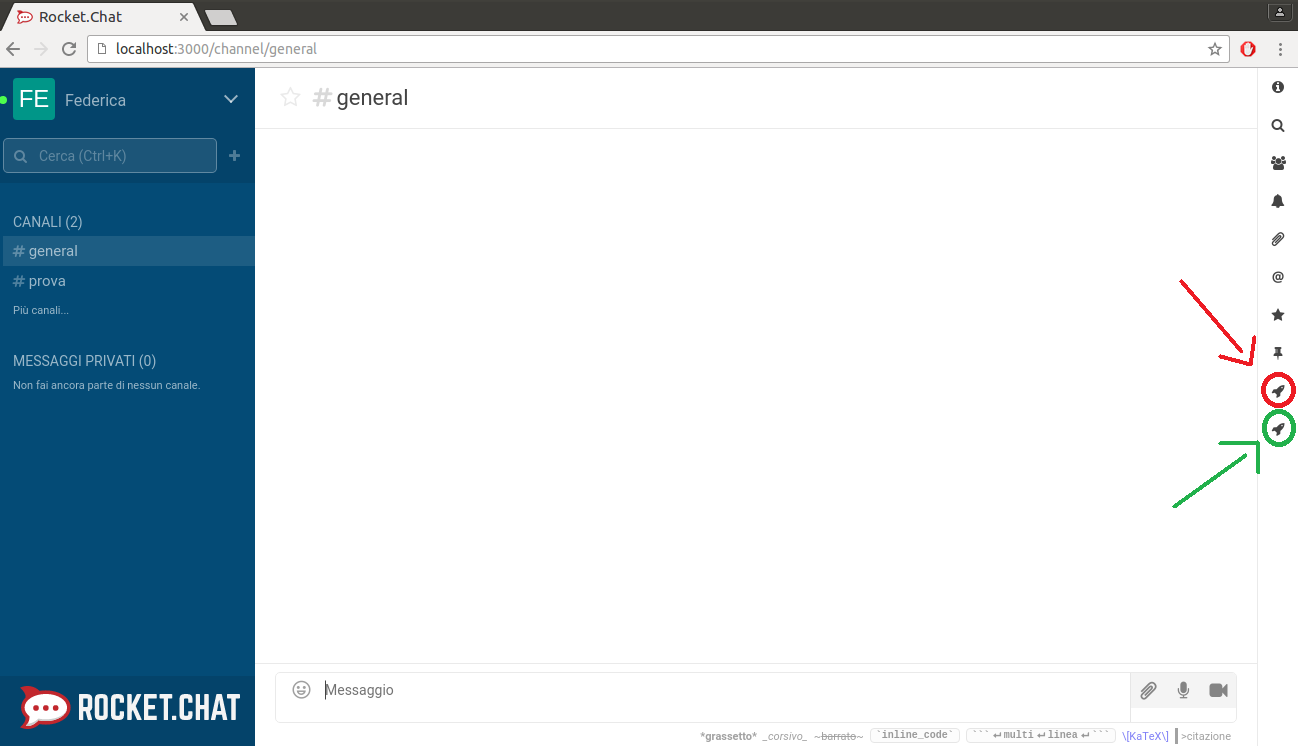
\includegraphics[scale=0.23]{img/f3.png}
		\end{center}
	\end{figure}	
\end{frame}

\begin{frame}
  
  \begin{center}
  	\begin{figure}
 		\caption{Storico delle bolle inviate e creazione di una nuova bolla}
  		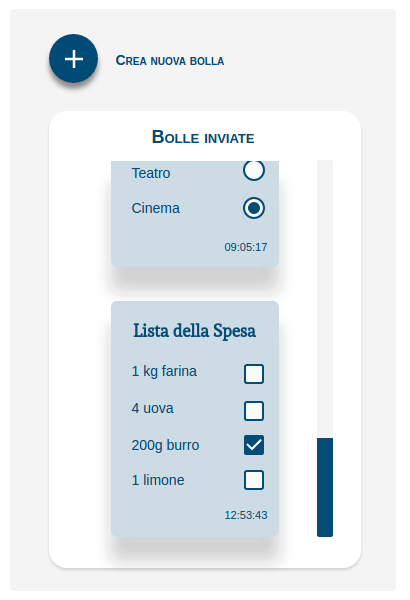
\includegraphics[scale=0.34]{img/mockup_1.png}
  	\end{figure}
  \end{center}
% \footnote{pie di pagina}
  
\end{frame}

\begin{frame}
	\begin{figure}
		\begin{center}
			\caption{Menù dei tipi di bolla}
			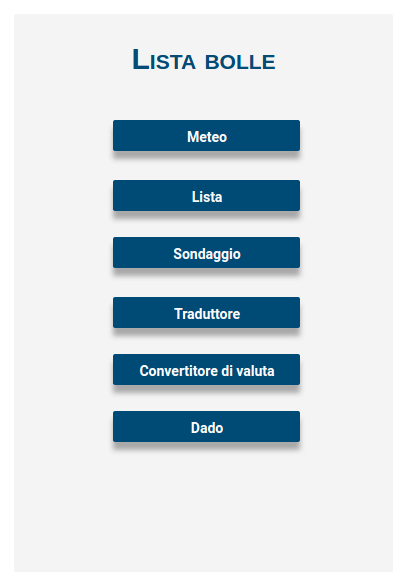
\includegraphics[scale=0.35]{img/mockup_2.png}
		\end{center}
	\end{figure}	
\end{frame}

\begin{frame}
	\begin{figure}
		\begin{center}
			\caption{Menù di configurazione di una bolla}
			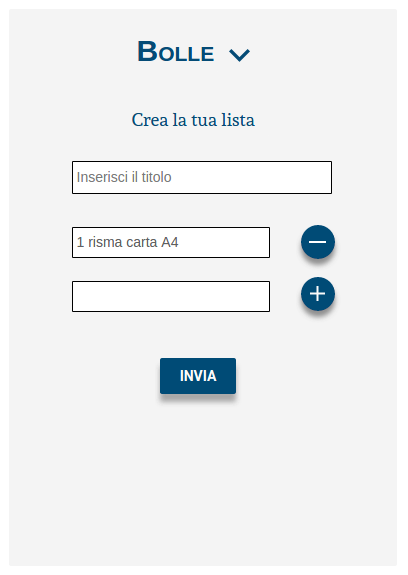
\includegraphics[scale=0.35]{img/mockup_3.png}
		\end{center}
	\end{figure}	
\end{frame}

\begin{frame}
	\begin{figure}
		\begin{center}
			\caption{Due nuovi pulsanti nella tabbar laterale}
			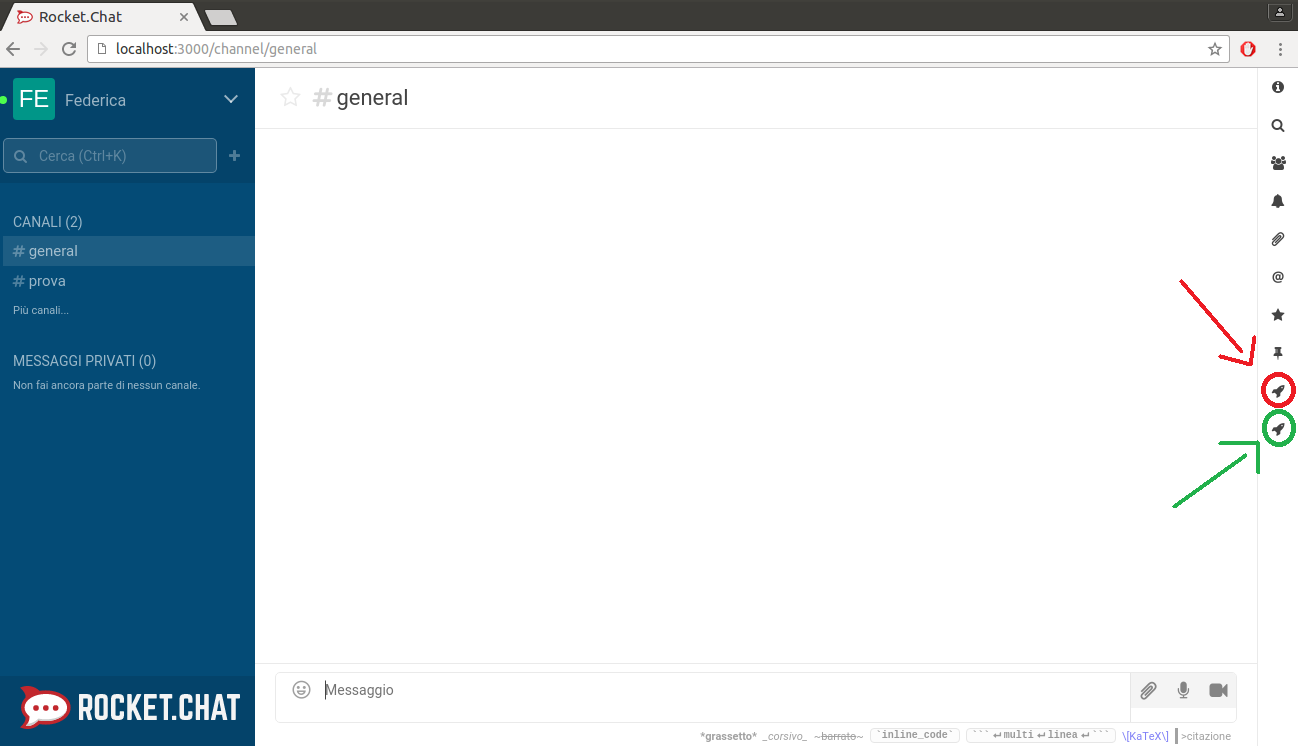
\includegraphics[scale=0.23]{img/f3.png}
		\end{center}
	\end{figure}	
\end{frame}

\begin{frame}
	\begin{figure}
		\begin{center}
			\caption{Storico delle bolle ricevute}
			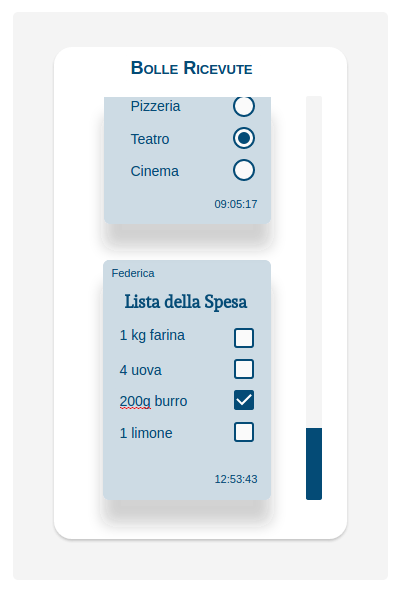
\includegraphics[scale=0.35]{img/mockup_4.png}
		\end{center}
	\end{figure}	
\end{frame}

\begin{frame}
\frametitle{Vantaggi}	
	\begin{columns}
		\begin{column}{0.2\textwidth}
			
		\end{column}
		
		\begin{column}{0.4\textwidth}
		%	\textbf{Vantaggi}:
			\begin{itemize}
				\item Bolle indipendenti dai messaggi
				\item Configurazione della bolla in spazio adeguato
				\item Interfaccia responsive
			\end{itemize}
		\end{column}
		
		\begin{column}{0.2\textwidth}
			
		\end{column}
	\end{columns}
	
\end{frame}
